\scanpage{6}
They correspond to the subgroups \inserted{$H$} of $\mathbb{Z}$, distinct from $\mathbb{Z}$ ($c=\operatorname{card}\mathbb{Z}/H$).....

\uline{Orientation of a contour} : \deleted{\unsure{Ch.|En.}}

\uline{Proposition} Let\deleted{\unsure{s|x}} $X=(S,A,R)$ be a connected \inserted{\deleted{\unsure{strict}}} contour $\ne\phi$.

% Two drawings in the left margin: the coordinates preserve the separate
% black lens and blue pentagon, including the small retracings at the corners.
\figure{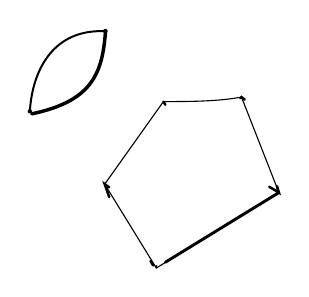
\begin{tikzpicture}[x=.0082cm,y=-.0082cm,line cap=round]
\draw[line width=.72pt] (5,126) .. controls (9,60) and (43,-2) .. (122,2);
\draw[line width=1.25pt] (122,5) .. controls (117,71) and (98,111) .. (8,130);
\fill (5,126) circle[radius=3.4]; \fill (122,2) circle[radius=3.7];
\draw (121,239) -- (212,111) .. controls (249,111) and (297,111) .. (333,104)
  -- (391,252) -- (201,369) -- cycle;
\draw[line width=1.05pt] (215,360) -- (391,252);
\draw[line width=.9pt] (128,244)--(121,239)--(128,259)
  (212,111)--(215,116)
  (331,106)--(333,104)--(338,108) (376,243)--(391,252)--(388,242)
  (192,358)--(196,365);
\fill (201,366) circle[radius=1.8];
\end{tikzpicture}}

a) \deleted{\unsure{An}}\inserted{Let $g$ be an} automorphism $g$ of $X$ \deleted{\unsure{is} \unsure{called} \uline{\unsure{direct}}.}\inserted{Equivalent conditions.}
\margin{\uuline{of orientation}}

$1^{\circ})$ \deleted{\unsure{if}} $\forall s\in S$, $s$ is linked to $gs$

$2^{\circ})$ $\forall a\in A\quad ga$ is linked to $a$

\deleted{\unsure{$\{$|$f$}}

\deleted{\unsure{b)|If}} We say that $g$ is an \deleted{\unsure{automorphism} of }\uline{orientation} of $X$.

b) Let $\omega(X)$\inserted{$\subset\operatorname{Aut}(X)$} be the set of \deleted{\unsure{automorphisms} of }\unsure{orientations|orientation} of $X$

\inserted{If $g\in\omega(X)$, we have $g^{-1}\in\omega(X)$.}

Then $\operatorname{card}\omega(X)=2$ \unsure{;|,} \deleted{\unsure{and} \unsure{if} $\unsure{g\in\omega|g\in\omega(X)}$} \inserted{(if $X$ is strict i.e. if $\unsure{c|(}=\operatorname{card}S\ne2$)} , and if $g\in\omega(X)$, we have $\omega(X)=\{g,g^{-1}\}$.

c) \deleted{Let $\operatorname{Aut}^{+}(X)\subset\operatorname{Aut}(X)$ be the \unsure{subgroup} of $\operatorname{Aut}X$ \unsure{formed} by the $\unsure{g\in\operatorname{Aut}X}$ such that $g$ acts \unsure{trivial$^{\mathrm{ly}}$|trivial$^{\mathrm{ly}}$} on $\omega(X)$ [i.e.}

Consider $\operatorname{Aut}(X)\unsure{-|\to}\operatorname{Aut}(\omega(X))\simeq\mathbb{Z}/2\mathbb{Z}$.

This is a surjective homomorphism, i.e. the kernel $\operatorname{Aut}^{+}(X)$ is a subgroup of index $2$.

Moreover, $\operatorname{Aut}^{+}(X)$ is a cyclic group generated by every $g\in\omega(X)$.

\uline{Corollary} $\operatorname{Aut}(X)\simeq\mathbb{Z}/2\mathbb{Z}\cdot\mathbb{Z}/H$ \inserted{($\frac{1}{2}$-direct \unsure{product|products}):}, where $H$ \unsure{is|$\to$} the subgroup of $\mathbb{Z}$ formed by the $n\in\mathbb{Z}$ such that $g^{n}=1$ ($g$ \unsure{being|being|being|in} a \unsure{fixed|fixed} orientation)
% archive sheet number: 5
